\section{rsyslog}
\subsection{Installation}
In einigen Linux Distributionen wie zum Beispiel Debian und Ubuntu ist rsyslog schon zum Standard geworden. Für andere Distributionen empfiehlt es sich den Paketmanager zur Installation zu verwenden.

\begin{tabular}{ll}
	\hline
	Linux Distribution & Installationsbefehl\\
	\hline\hline
	Debian, Ubuntu & apt-get install rsyslog\\
	SUSE, openSUSE & yast -i rsyslog\\
	Fedora         & yum install rsyslog\\
	Gentoo         & emerge rsyslog
\end{tabular}

\begin{informationnote}
	Gentoo Benutzer sollten die passenden Useflags für das rsyslog Paket beachten. Empfehlenswert sind
	\textit{gnutls}, \textit{logrotate} und \textit{zlib}. 
\end{informationnote}

\subsection{Allgemeine Konfiguration}
Mit rsyslog ist eine sehr umfangreiche Konfiguration möglich. Es können Nachrichten nach regulären Ausdrücken analysiert und in bestimmte Protokolldateien geschrieben werden.

Die Konfiguration des rsyslog-Dienstes erfolgt auf Debian basierten Distributionen in \textit{/etc/rsyslog.conf} und \textit{/etc/rsyslog.d/*.conf}.

\subsubsection{Erklärung der Standardkonfiguration}
Die Konfiguration kann im bekannten syslog-BSD-Syntax vorgenommen werden. Rsyslog besteht aus Modulen, diese können per \textit{\$ModLoad} aktiviert werden. Eine Liste aller Module kann auf der rsyslog Internetseite nachgelesen werden \url{http://www.rsyslog.com/doc/rsyslog_conf_modules.html}.

Der Syntax für das Protokollieren eines Dienstes ist wie folgt aufgebaut.
\begin{lstlisting}
Dienst.Gewichtung -/pfad/zur/log/datei.log
\end{lstlisting}

Beispiel für das Mail-Protokollieren nach Gewichtung:
\begin{lstlisting}
mail.info           -/var/log/mail.info
mail.warn           -/var/log/mail.warn
mail.err            /var/log/mail.err
\end{lstlisting}

Durch das Minus wird festgelegt, dass die Protokolldatei nach jedem Loggen synchronisiert wird. Der genaue Syntax für das Filtern der Informationen findet man auf rsyslog Internetseite \url{http://www.rsyslog.com/doc/rsyslog_conf_actions.html}

\subsubsection{Filtern nach Programmname}
Eine einfache und sinnvolle Anpassung für rsyslog ist die automatische Filterung nach einem Programmname. Hierzu wird ein Template erstellt und das komplette Logging darauf umgeleitet.

\begin{lstlisting}
$template PerAppLogs,"/var/log/rsyslog/%programname%.log"
# Per application log file
*.*  -?PerAppLogs
\end{lstlisting}

\subsection{Remote Logging Konfiguration}
% TODO: Ein zwei Sätze zum Remote Logging

\subsubsection{Server}
Um das Remote Logging zu aktivieren müssen folgende Zeilen in der \textit{/etc/rsyslog.conf} auskommentiert oder hinzugefügt werden:

\begin{lstlisting}
$ModLoad imudp
$UDPServerRun 514
\end{lstlisting}

Bei UDP Port 514 handelt es sich um den Standard syslog-Port. Es ist zu beachten das dieser Port in der Firewall freigeschaltet wurde.

Um entsprechende Zugriffsrechte für den eigenen Server oder das gesamte Subnetz festzulegen wird eine Datei \textit{/etc/rsyslog.d/00-AllowRemoteLogging.conf} angelegt. In dieser kann nun per \textit{\$AllowedSender} der Zugriff gesteuert werden.

\begin{informationnote}
Es wird Empfohlen die Konfiguration in mehrere, nach Teilaufgaben spezifizierte, Dateien aufzuteilen.
\end{informationnote}

\begin{lstlisting}
# Ein Host
$AllowedSender UDP, 192.168.56.100
# Alle Hosts aus einem Subnetz
$AllowedSender UDP, 192.168.56.0/24
# Jeder von kernel.org
$AllowedSender UDP, *.kernel.org
\end{lstlisting}

Folgende Verzeichnis Struktur ist für die Protokolldateien gewünscht. Die Ordner müssen hierzu jedoch angelegt werden. Es ist gewünscht das pro Server eine Protokolldatei in \textit{/var/log/rsyslog.remote/\%HOSTNAME\%.log} existiert.

\begin{itemize}
\item /var/log/rsyslog.remote/
\item /var/log/rsyslog.remote.archive/
\end{itemize}

Um die oben genannte Protokolldatei pro Server zu erhalten, ist eine Anpassung der \textit{\$template} in der \textit{/etc/rsyslog.d/01-RemoteTemplate.conf} nötig. \cite{RsyslogSeparateLog}

\begin{lstlisting}
$template RemoteServerLog, "/var/log/rsyslog.remote/%HOSTNAME%.log"
*.* -?RemoteServerLog
\end{lstlisting}

\subsubsection{Linux Client}
Es erfolgt nun die Konfiguration eines Linux Client Rechners. Dieser soll all seine Protokollinformationen an den Server senden. Hierzu ist ein einfacher Eintrag in \textit{/etc/rsyslog.d/00-RemoteLogging.conf} nötig.

\begin{lstlisting}
*.*	@192.168.56.1
\end{lstlisting}

Ein \textit{@}-Zeichen gibt an das die Protokollinformationen per UDP an den Server versandt werden. Um eine TCP Verbindung zu verwenden müssen zwei \textit{@}-Zeichen verwendet werden.

\begin{importantnote}
Nach einer Konfigurationsänderung muss der rsyslog-Dienst neu gestartet werden. Dies erfolgt mit \textit{/etc/init.d/rsyslog restart}. Administrationsrechte sind hierzu erforderlich.
\end{importantnote}

\subsubsection{Windows Client}
Standardmäßig unterstützt Windows das syslog-Protokoll nicht. Abhilfe schafft SysLogAgent, eine kommerzielle Anwendung von Datagram Consulting. Die Software kann kostenlos auf \url{http://syslogserver.com/syslogagent.html} heruntergeladen werden.

\begin{figure}[h]
\begin{center}
 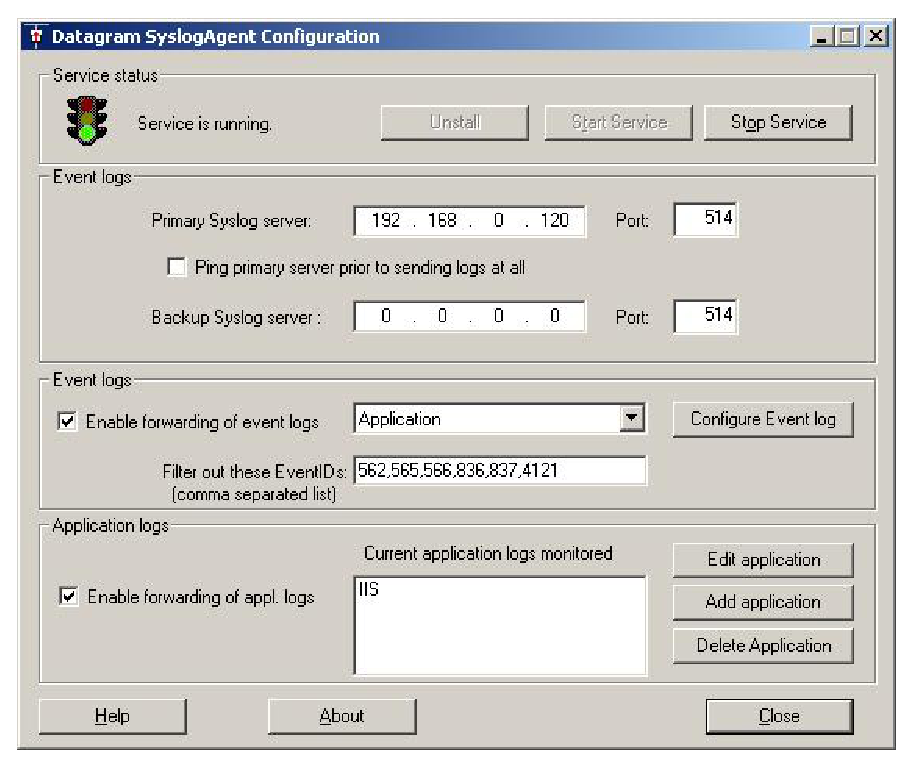
\includegraphics[width=\textwidth]{content/images/syslogagent.eps}
  \caption{SysLogAgent Konfiguration - Quelle: \cite{SysLogAgentScreendump}}
\end{center}
\end{figure}

Nach einer erfolgreichen Installation und dem Start des Dienstes kann in der GUI die IP-Adresse des rsyslog-Servers eingetragen werden. Ein eigenes Ereignis kann per Kommandozeile versandt werden.

\begin{lstlisting}
eventcreate /t ERROR /id 666 /d "Diese Windows Lizenz ist abgelaufen!"
\end{lstlisting}
